\documentclass[12pt]{article}

\usepackage{sbc-template}
\usepackage{graphicx}
\usepackage[utf8]{inputenc}
\usepackage[brazil]{babel}
\usepackage{url}
\usepackage{booktabs}
\usepackage{float}

\sloppy

\title{Análise de Perfis de Risco em Saúde Materna por Clusterização Não Supervisionada}

\author{Gabriel Stiegemeier\inst{1}, Guilherme Einloft\inst{1}}

\address{Universidade Federal de Santa Maria\\
  Santa Maria, RS, Brasil
  \email{\{gstiegemeier, geinloft\}@inf.ufsm.br}
}

\begin{document}

\maketitle



\section{Introdução}

Neste projeto, aplicamos técnicas de aprendizado não supervisionado para explorar o \textbf{Maternal Health Risk Data Set}, um conjunto de dados público focado na saúde de gestantes. O dataset está disponível no UCI Machine Learning Repository e no Kaggle, e foi originalmente analisado no artigo de \cite{ahmed2020review}. A ideia central é investigar o comportamento de algoritmos clássicos de clusterização diante de dados reais e fisiológicos.

\subsection{Justificativa da Escolha do Dataset}

Embora a especificação do trabalho prático liste como exemplos de domínio \textit{Diabetes, Doença Cardiovascular ou Hipertensão}, o dataset \textbf{Maternal Health Risk} foi escolhido por ser \textbf{diretamente fundamentado nessas mesmas condições clínicas}. Das seis variáveis preditoras do dataset, três são marcadores centrais dessas patologias:

\begin{itemize}
    \item \textbf{SystolicBP e DiastolicBP (Pressão Arterial Sistólica e Diastólica):} São os indicadores primários para diagnóstico de \textbf{hipertensão gestacional} e \textbf{pré-eclâmpsia}, condições hipertensivas que afetam 5--8\% das gestações e representam uma das principais causas de mortalidade materna. Os limiares diagnósticos (PA $\geq$ 140/90 mmHg) estão diretamente representados nos dados.
    \item \textbf{BS (Blood Sugar --- Glicemia):} É o marcador fundamental para diagnóstico de \textbf{diabetes mellitus gestacional (DMG)}, condição que acomete 7--14\% das gestações. Valores elevados de BS no dataset correspondem diretamente aos critérios diagnósticos de diabetes.
\end{itemize}

Portanto, apesar de o dataset ter como tema a saúde materna, \textbf{as variáveis utilizadas e os perfis de risco investigados são intrinsecamente ligados à hipertensão e ao diabetes} --- duas das três condições explicitamente mencionadas na especificação. O clustering aplicado neste trabalho busca, na prática, identificar subgrupos de pacientes com perfis hipertensivos e/ou diabéticos.

Além disso, o dataset atende a todos os critérios técnicos exigidos: é real, possui mais de 1.000 instâncias e foi utilizado em artigo científico publicado.

\subsection{Definição do Problema}

\textbf{Tese:} Investigar se algoritmos de clustering não supervisionados conseguem agrupar naturalmente gestantes em perfis de risco (alto, médio, baixo) utilizando exclusivamente métricas fisiológicas --- como pressão arterial, níveis de glicose, idade, temperatura corporal e frequência cardíaca --- sem que o algoritmo tenha acesso ao diagnóstico prévio.

Essa investigação é relevante porque, caso os algoritmos consigam formar agrupamentos que correspondam aos níveis de risco previamente diagnosticados por especialistas, isso validaria a existência de \textbf{padrões fisiológicos naturais} que distinguem gestantes de alto, médio e baixo risco.

\textbf{Hipóteses formais:}
\begin{itemize}
    \item \textbf{H1:} Os algoritmos de clusterização formarão agrupamentos que correspondem aos três níveis de risco originais (alto, médio e baixo), indicando que as métricas fisiológicas disponíveis são suficientes para estratificar gestantes.
    \item \textbf{H2:} O cluster de alto risco será o mais distinguível dos três, apresentando a maior pureza na correspondência com o rótulo original, dado que as condições de alto risco (hipertensão severa, diabetes descompensado) envolvem alterações fisiológicas mais pronunciadas.
\end{itemize}

\subsection{Descrição do Dataset}

O dataset é composto por \textbf{1.014 registros} coletados por meio de dispositivos IoT (Internet of Things) e sistemas hospitalares, contendo as variáveis apresentadas na Tabela \ref{tab:dataset_desc}.

\begin{table}[H]
\centering
\caption{Descrição das Variáveis do Dataset}
\label{tab:dataset_desc}
\begin{tabular}{lll}
\toprule
\textbf{Variável} & \textbf{Tipo} & \textbf{Descrição} \\
\midrule
Age & int & Idade da gestante (anos) \\
SystolicBP & int & Pressão arterial sistólica (mmHg) \\
DiastolicBP & int & Pressão arterial diastólica (mmHg) \\
BS & float & Nível de glicose no sangue (mmol/L) \\
BodyTemp & float & Temperatura corporal (Fahrenheit) \\
HeartRate & int & Frequência cardíaca (bpm) \\
RiskLevel & string & Nível de risco: low risk, mid risk, high risk \\
\bottomrule
\end{tabular}
\end{table}

A distribuição original dos rótulos é de 406 para Low Risk (40.0\%), 336 para Mid Risk (33.1\%) e 272 para High Risk (26.8\%). 

\textit{Nota: A coluna RiskLevel foi utilizada apenas na Análise Descritiva para contextualização e na etapa final de Interpretação para validação dos clusters. Ela foi removida antes de qualquer etapa de modelagem, respeitando o caráter não supervisionado dos algoritmos.}

\section{Análise Descritiva (EDA)}

\subsection{Análise Univariada}

A Tabela \ref{tab:descritiva} resume as estatísticas descritivas de todas as variáveis numéricas:

\begin{table}[H]
\centering
\caption{Estatísticas Descritivas das Variáveis Numéricas}
\label{tab:descritiva}
\resizebox{\textwidth}{!}{%
\begin{tabular}{lrrrrrrrrr}
\toprule
\textbf{Variável} & \textbf{Média} & \textbf{Mediana} & \textbf{Desvio Padrão} & \textbf{Mín} & \textbf{Q1} & \textbf{Q3} & \textbf{Máx} & \textbf{IQR} \\
\midrule
Age & 29.87 & 26.0 & 13.47 & 10 & 19 & 39 & 70 & 20 \\
SystolicBP & 113.20 & 120.0 & 18.40 & 70 & 100 & 120 & 160 & 20 \\
DiastolicBP & 76.46 & 80.0 & 13.89 & 49 & 65 & 90 & 100 & 25 \\
BS & 8.73 & 7.5 & 3.29 & 6 & 6.9 & 8.0 & 19 & 1.1 \\
BodyTemp & 98.67 & 98.0 & 1.37 & 98 & 98 & 98 & 103 & 0 \\
HeartRate & 74.30 & 76.0 & 8.09 & 7 & 70 & 80 & 90 & 10 \\
\bottomrule
\end{tabular}%
}
\end{table}

\textbf{Observações-chave da análise univariada:}
\begin{itemize}
    \item \textbf{Age:} Distribuição assimétrica à direita (média $>$ mediana), com amplitude de 10 a 70 anos, indicando grande diversidade etária no dataset.
    \item \textbf{SystolicBP e DiastolicBP:} Apresentam correlação forte entre si (detalhado na análise bivariada). A sistólica concentra-se em torno de 120 mmHg.
    \item \textbf{BS (Glicose):} Fortemente assimétrica à direita, com mediana 7.5 e média 8.73, indicando que a maioria das gestantes apresenta níveis normais, mas há um subgrupo com glicose elevada (até 19 mmol/L).
    \item \textbf{BodyTemp:} Concentração extrema em 98.0 $^\circ$F, com IQR = 0, indicando baixa variabilidade. Valores acima de 100 $^\circ$F sugerem condições febris.
    \item \textbf{HeartRate:} Foram identificados \textbf{2 registros com HeartRate = 7 bpm}, valores fisiologicamente impossíveis que representam erros de digitação. Esses registros foram tratados na etapa de pré-processamento.
\end{itemize}

As Figuras \ref{fig:histogramas} e \ref{fig:boxplots} ilustram a distribuição das variáveis.

\begin{figure}[H]
    \centering
    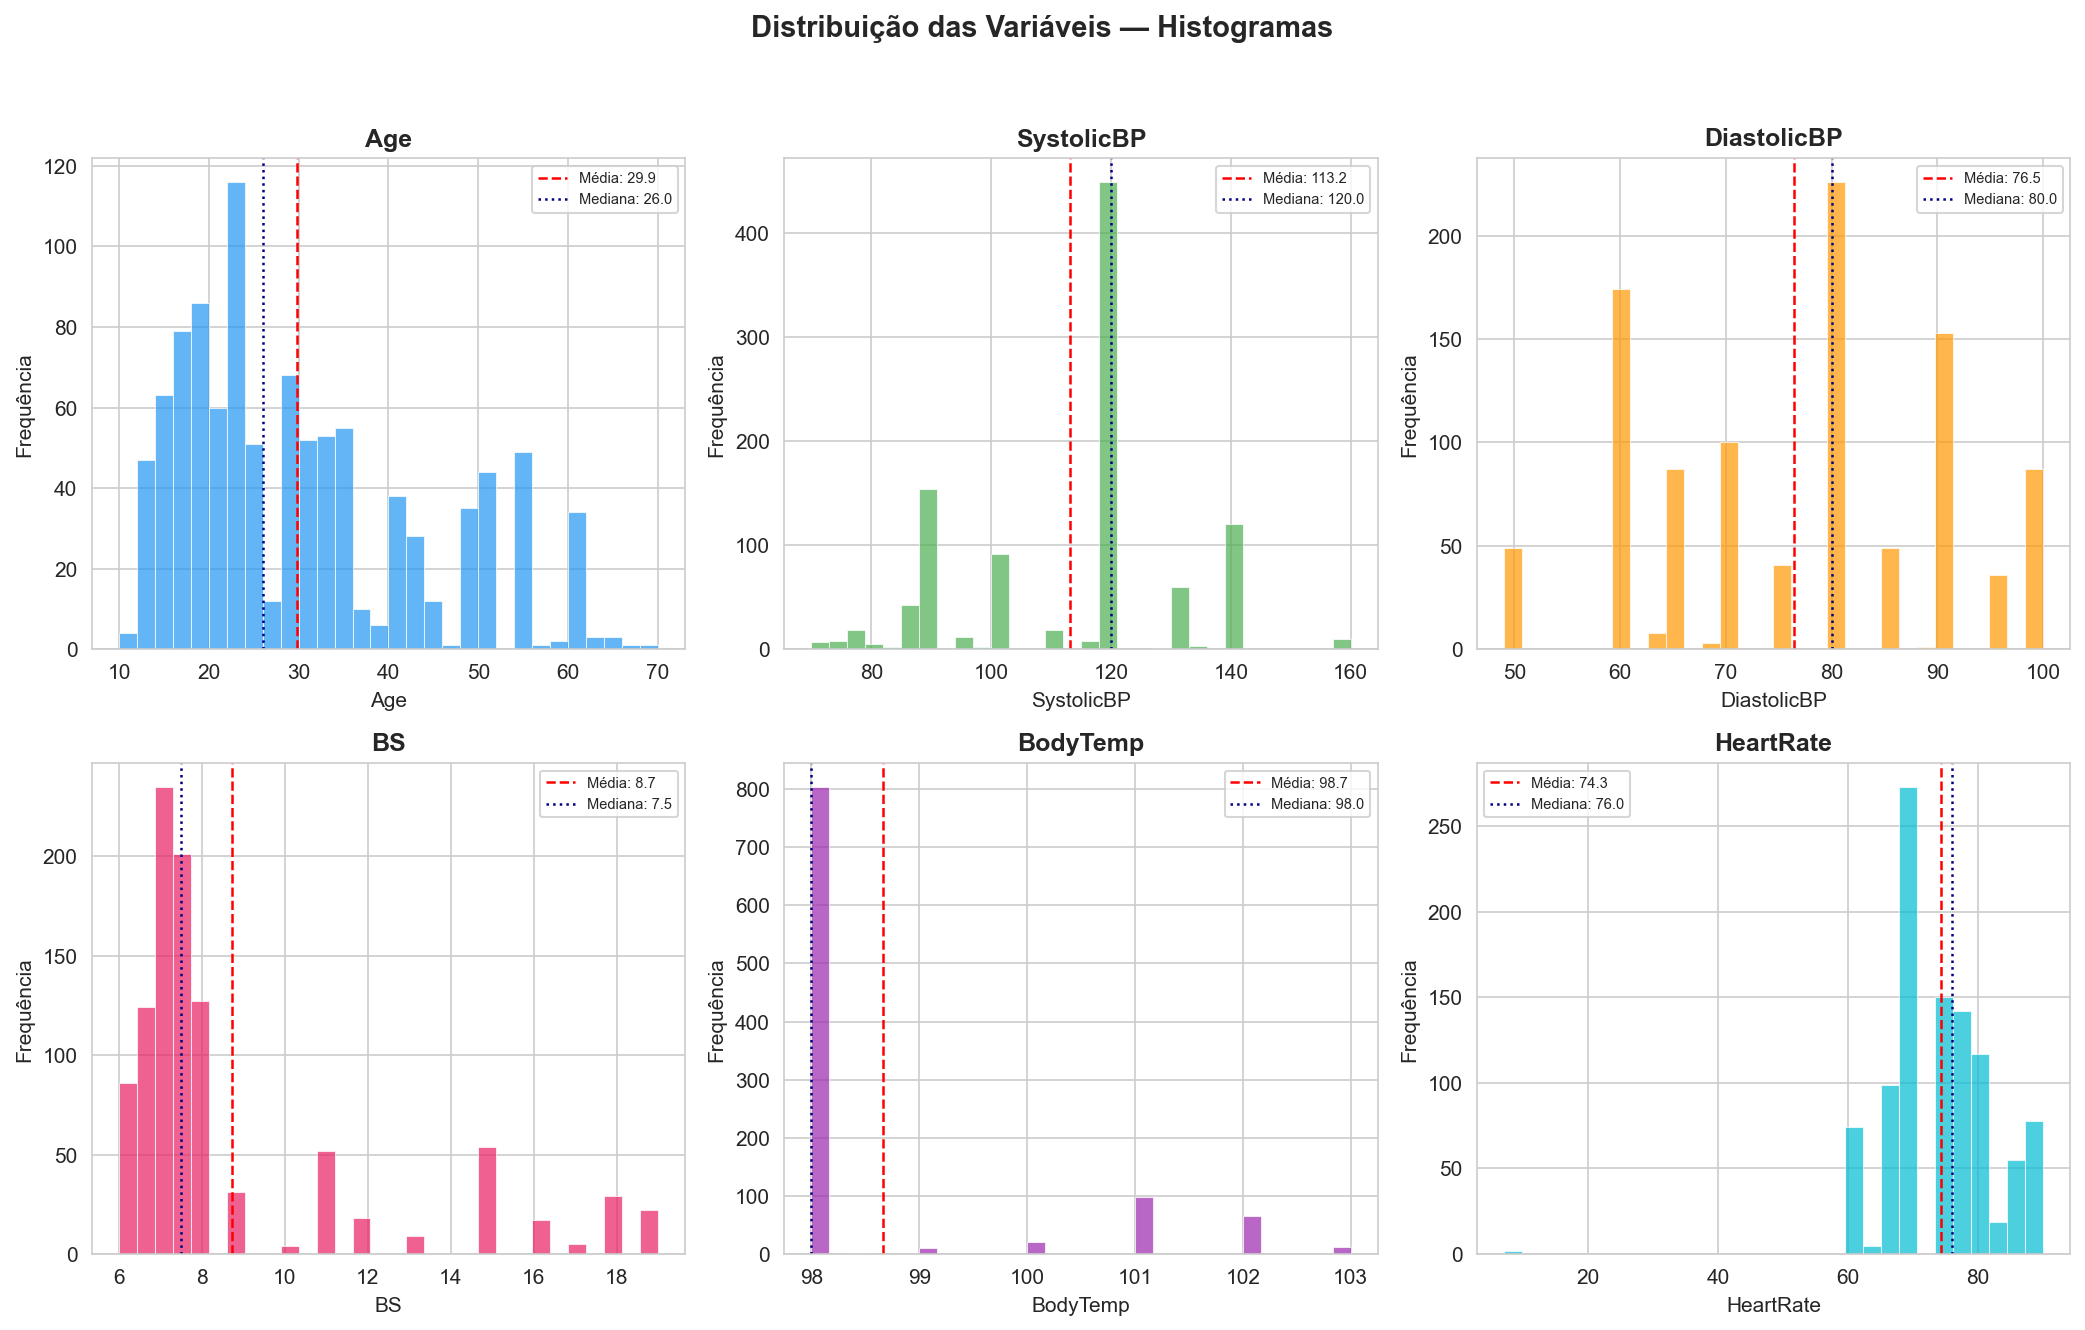
\includegraphics[width=\textwidth]{graficos/01_histogramas.png}
    \caption{Distribuição das Variáveis --- Histogramas}
    \label{fig:histogramas}
\end{figure}

\begin{figure}[H]
    \centering
    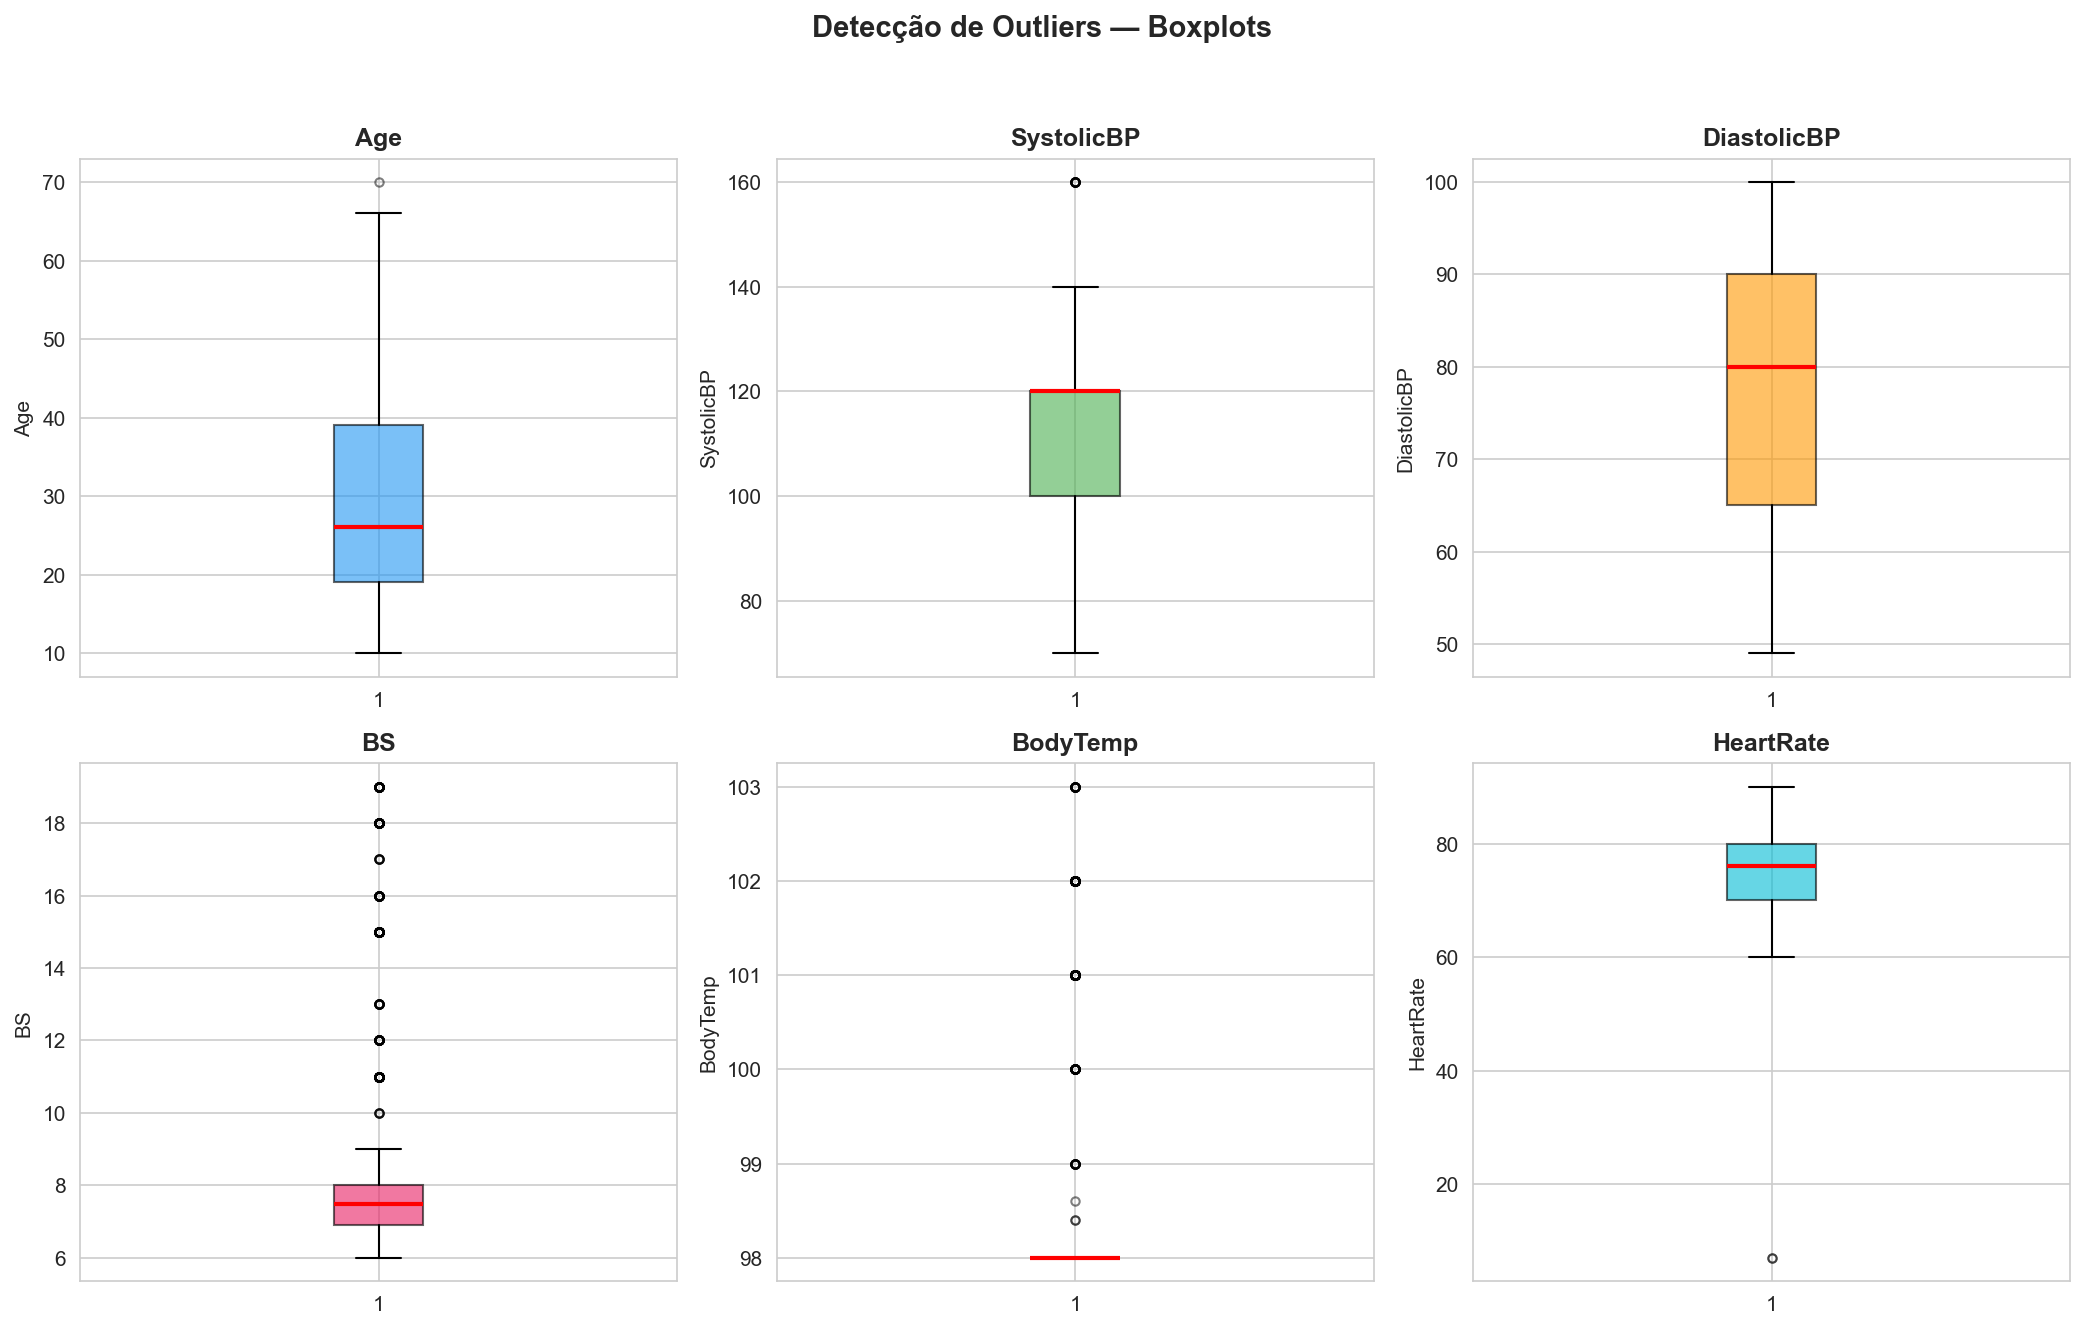
\includegraphics[width=\textwidth]{graficos/02_boxplots.png}
    \caption{Detecção de Outliers --- Boxplots}
    \label{fig:boxplots}
\end{figure}

\subsection{Análise Bivariada}

As matrizes de correlação (Pearson e Spearman) revelaram as seguintes relações mais relevantes (Tabela \ref{tab:correlacoes}):

\begin{table}[H]
\centering
\caption{Principais Correlações Bivariadas}
\label{tab:correlacoes}
\begin{tabular}{lrrl}
\toprule
\textbf{Par de Variáveis} & \textbf{Pearson} & \textbf{Spearman} & \textbf{Interpretação} \\
\midrule
SystolicBP $\times$ DiastolicBP & \textbf{0.787} & \textbf{0.757} & Correlação forte e positiva \\
Age $\times$ BS & 0.473 & 0.320 & Correlação moderada \\
Age $\times$ SystolicBP & 0.416 & 0.485 & Correlação moderada \\
BS $\times$ SystolicBP & 0.425 & 0.262 & Correlação moderada \\
BodyTemp $\times$ Age & -0.255 & -0.305 & Correlação fraca negativa \\
HeartRate $\times$ BS & 0.143 & 0.129 & Correlação negligenciável \\
\bottomrule
\end{tabular}
\end{table}

\textbf{Observações:}
\begin{itemize}
    \item A forte correlação entre \textbf{SystolicBP e DiastolicBP} ($r = 0.787$) era esperada clinicamente, pois ambas representam componentes da pressão arterial.
    \item A correlação moderada entre \textbf{Age e BS} ($r = 0.473$) sugere que gestantes mais velhas tendem a apresentar níveis glicêmicos mais elevados.
    \item \textbf{HeartRate} apresenta correlação fraca com todas as outras variáveis, sugerindo que a frequência cardíaca atua como variável relativamente independente.
\end{itemize}

A Figura \ref{fig:scatter} ilustra o relacionamento bivariado por nível de risco.

\begin{figure}[H]
    \centering
    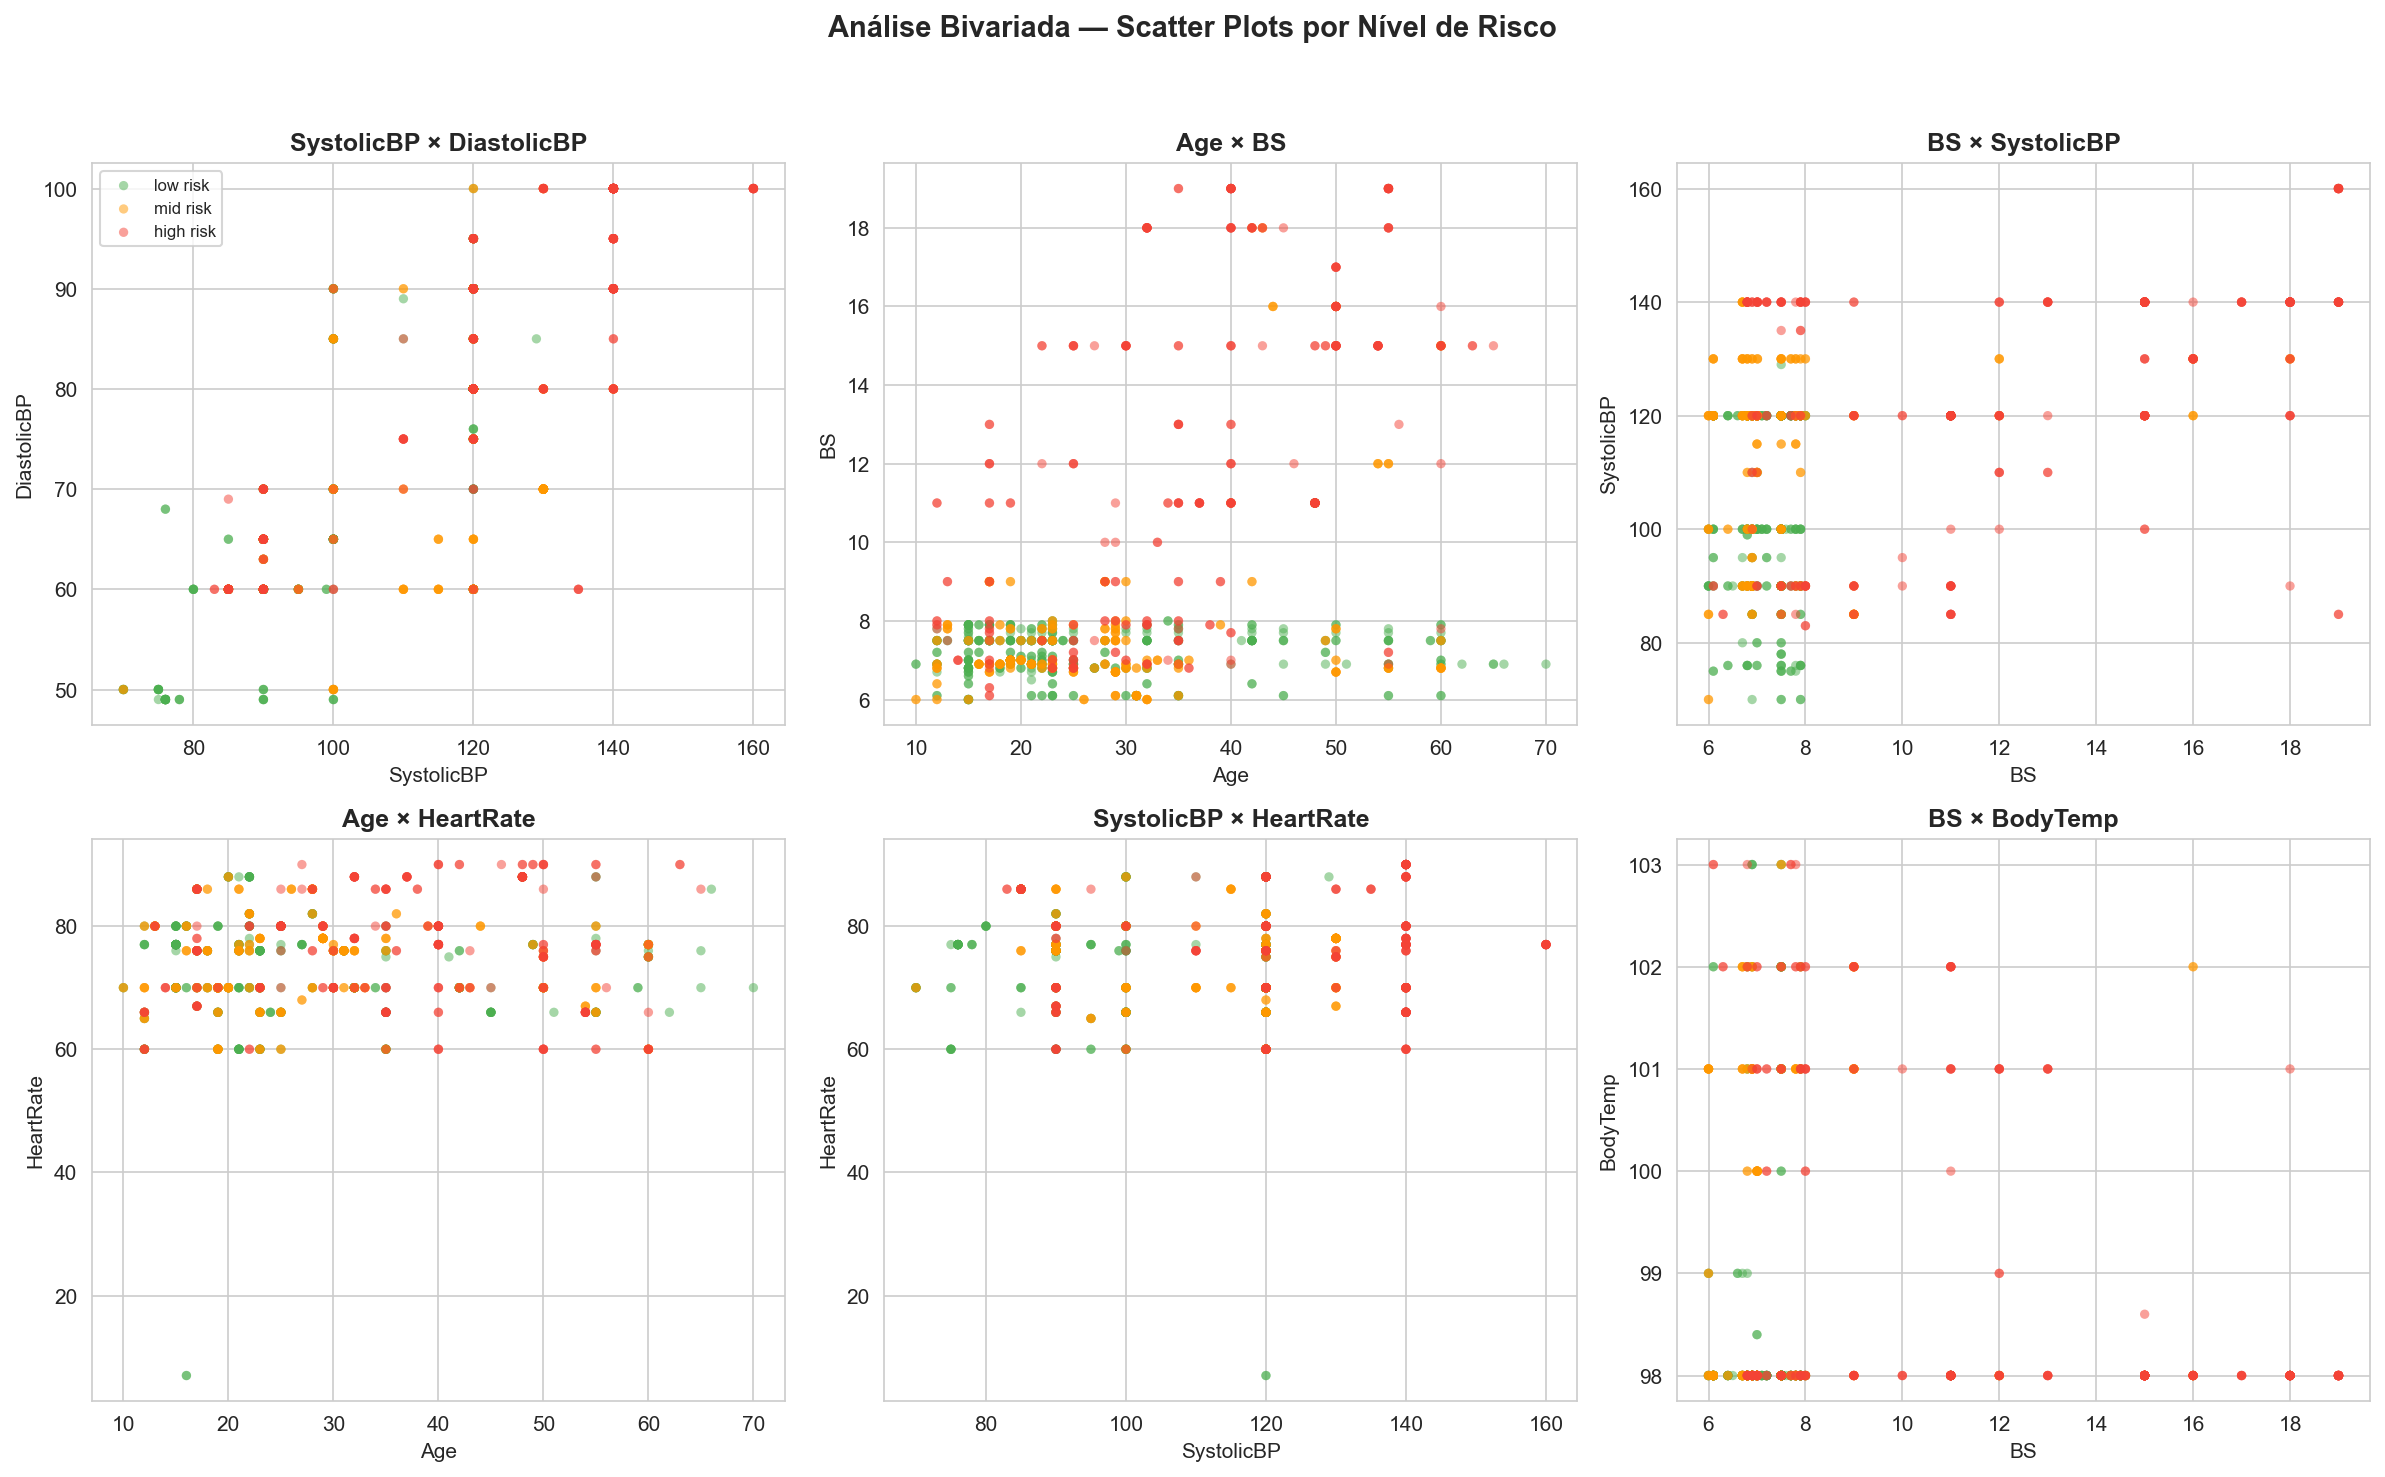
\includegraphics[width=\textwidth]{graficos/03_scatter_bivariada.png}
    \caption{Análise Bivariada --- Scatter Plots por Nível de Risco}
    \label{fig:scatter}
\end{figure}

\subsection{Análise Multivariada}

A \textbf{Análise de Componentes Principais (PCA)} foi aplicada aos dados padronizados para visualização bidimensional e análise da estrutura de variância do dataset. O \textbf{Scree Plot} (Tabela \ref{tab:scree} e Figura \ref{fig:scree}) mostra a contribuição individual e cumulativa de cada componente principal.

\begin{table}[H]
\centering
\caption{Variância Explicada por Componente (PCA)}
\label{tab:scree}
\begin{tabular}{lrr}
\toprule
\textbf{Componente} & \textbf{Variância Individual} & \textbf{Variância Cumulativa} \\
\midrule
PC1 & 43.5\% & 43.5\% \\
PC2 & 19.1\% & 62.5\% \\
PC3 & 14.0\% & 76.5\% \\
PC4 & 11.8\% & 88.3\% \\
PC5 & 8.2\% & 96.5\% \\
PC6 & 3.5\% & 100.0\% \\
\bottomrule
\end{tabular}
\end{table}

A análise do Scree Plot revela que \textbf{duas componentes explicam 62.5\% da variância total}, enquanto são necessárias \textbf{quatro componentes para atingir $\sim$88\%}. A escolha de 2 componentes para visualização é justificada pelo ponto de inflexão (cotovelo) observado entre PC2 e PC3.

\begin{figure}[H]
    \centering
    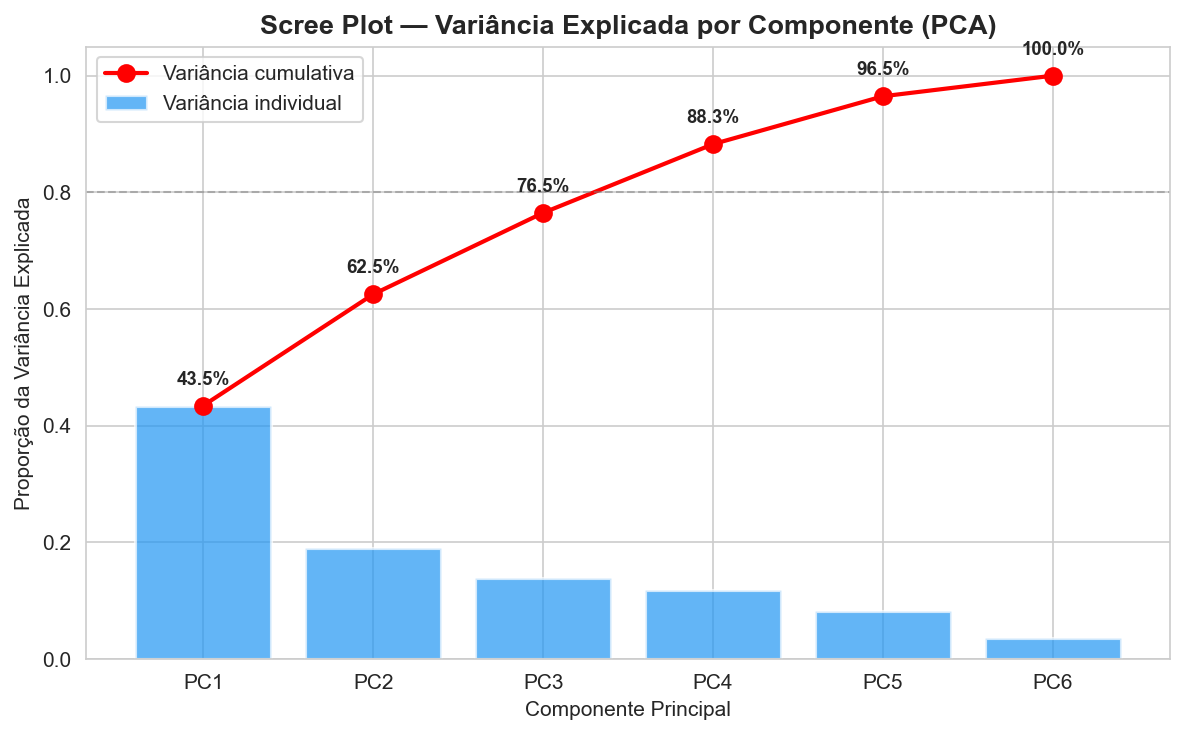
\includegraphics[width=0.75\textwidth]{graficos/05b_scree_plot.png}
    \caption{Scree Plot --- Variância Explicada por Componente}
    \label{fig:scree}
\end{figure}

A projeção PCA colorida pelos rótulos originais (RiskLevel) na Figura \ref{fig:pca_risco} revela que os grupos de risco apresentam \textbf{sobreposição considerável} no espaço bidimensional, com pontos de \textit{high risk} tendendo a se concentrar na região de valores positivos de PC1, enquanto \textit{low risk} tende para valores negativos. Essa sobreposição sugere que a separação entre os níveis de risco não é trivial e representa um desafio real para os algoritmos de clusterização. As correlações multivariadas também podem ser verificadas na Figura \ref{fig:heatmap}.

\begin{figure}[H]
    \centering
    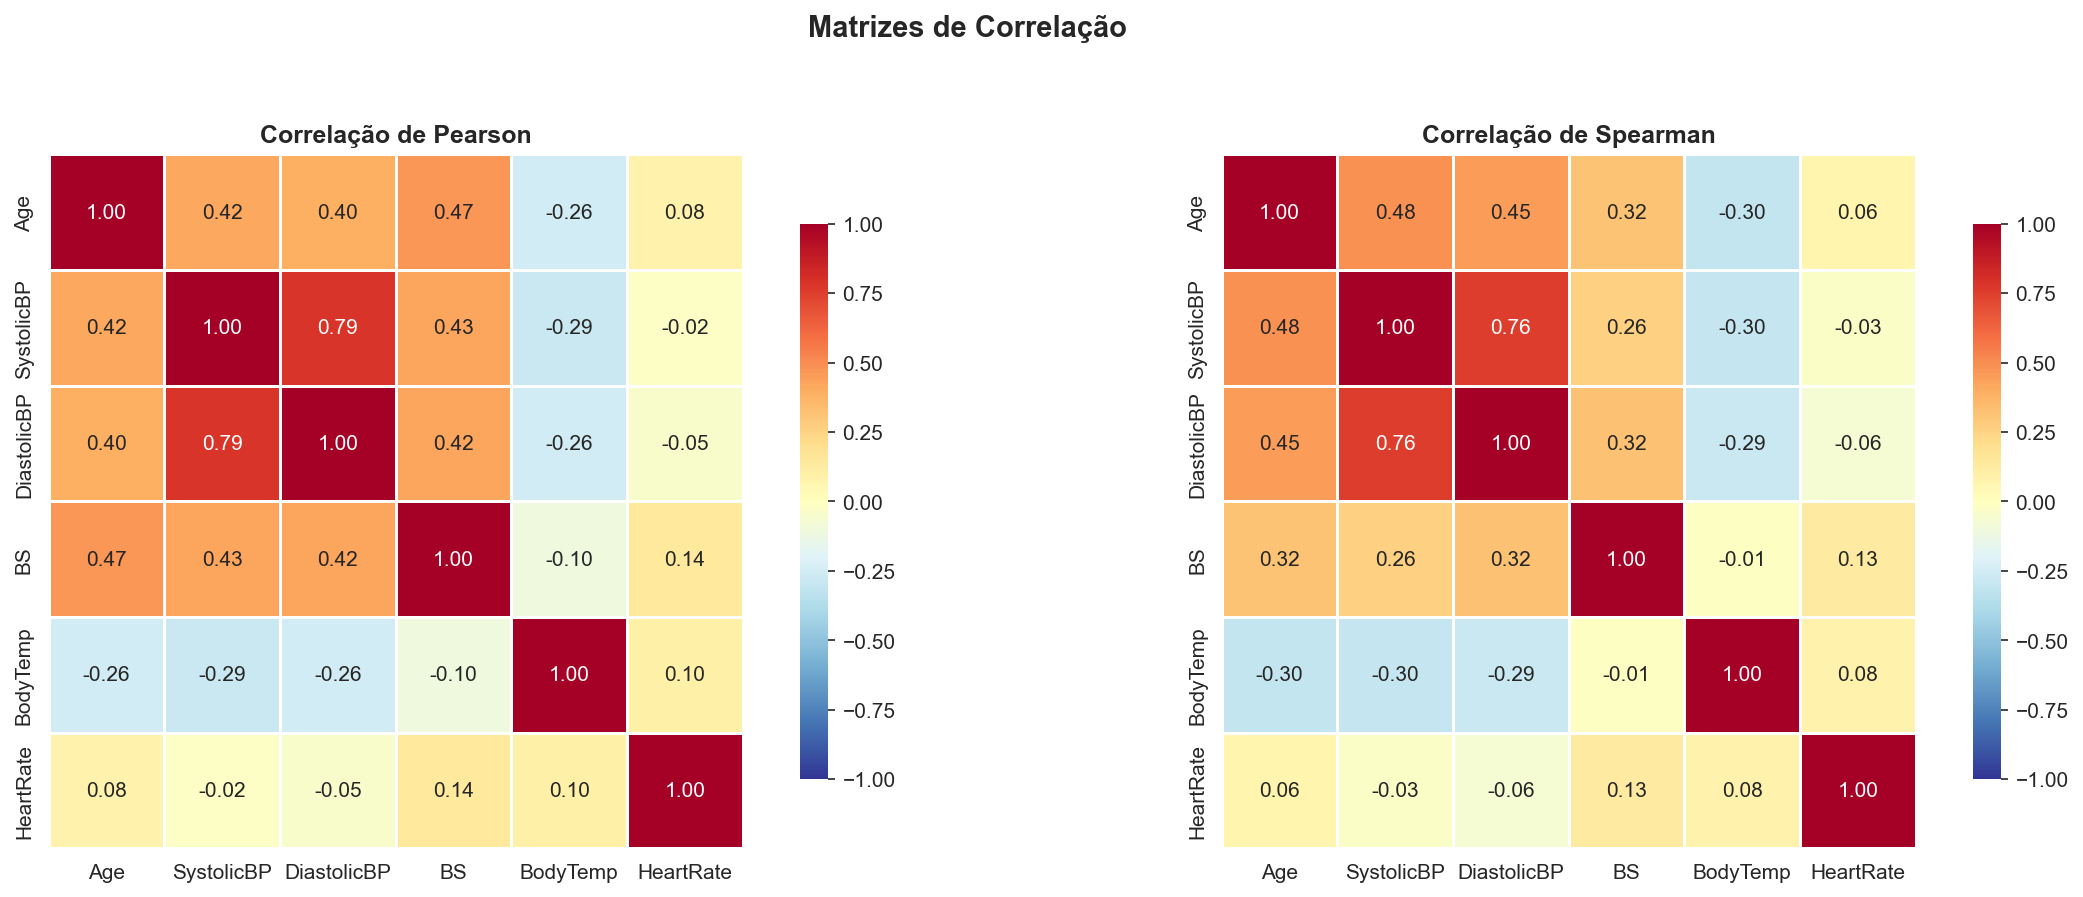
\includegraphics[width=0.8\textwidth]{graficos/04_heatmap_correlacao.png}
    \caption{Matrizes de Correlação --- Pearson e Spearman}
    \label{fig:heatmap}
\end{figure}

\begin{figure}[H]
    \centering
    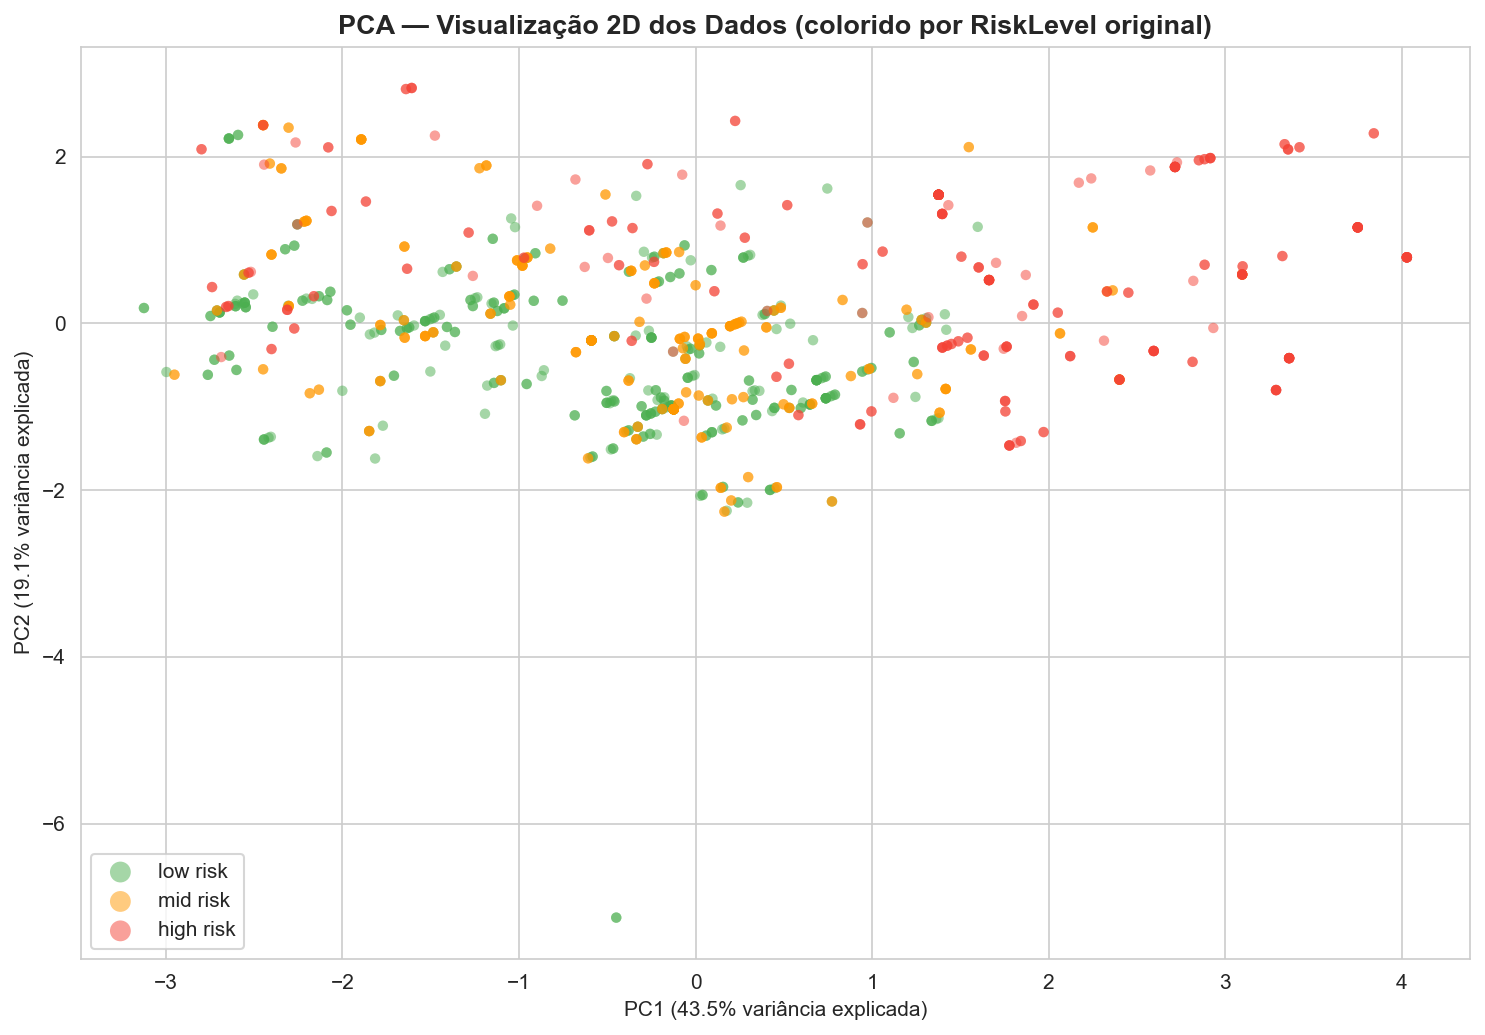
\includegraphics[width=0.8\textwidth]{graficos/05_pca_risklevel.png}
    \caption{PCA --- Visualização 2D dos Dados colorida por RiskLevel}
    \label{fig:pca_risco}
\end{figure}

\section{Pré-processamento}

\subsection{Tratamento de Valores Faltantes}
O dataset \textbf{não possui valores faltantes (NaN)} em nenhuma das colunas. Nenhum tratamento de imputação foi necessário.

\subsection{Remoção de Outliers Extremos (Erros de Digitação)}
Foram identificados \textbf{2 registros} com \texttt{HeartRate = 7 bpm}, um valor fisiologicamente impossível para seres humanos (a frequência cardíaca mínima viável em repouso é cerca de 40--50 bpm). Ambos os registros pertencem a uma gestante de 16 anos com as mesmas características (provavelmente o mesmo registro duplicado):

\begin{table}[H]
\centering
\caption{Registros com Erro de Digitação Removidos}
\label{tab:outliers_extremos}
\begin{tabular}{lrrrrrrl}
\toprule
\textbf{Age} & \textbf{SystolicBP} & \textbf{DiastolicBP} & \textbf{BS} & \textbf{BodyTemp} & \textbf{HeartRate} & \textbf{RiskLevel} \\
\midrule
16 & 120 & 75 & 7.9 & 98.0 & 7 & low risk \\
16 & 120 & 75 & 7.9 & 98.0 & 7 & low risk \\
\bottomrule
\end{tabular}
\end{table}

Esses registros foram \textbf{removidos do dataset} por serem claramente erros de digitação (provavelmente o valor correto seria 70 ou 77 bpm). Restaram \textbf{1.012 registros} após a remoção.

\subsection{Tratamento de Outliers via IQR}
Para as demais variáveis, foi aplicado o método de \textbf{clipping baseado no Intervalo Interquartil (IQR)}, que limita os valores ao intervalo $[Q1 - 1.5 \times IQR, Q3 + 1.5 \times IQR]$. A Tabela \ref{tab:clipping} resume a aplicação:

\begin{table}[H]
\centering
\caption{Limites de Clipping via IQR}
\label{tab:clipping}
\begin{tabular}{lrrr}
\toprule
\textbf{Variável} & \textbf{Limite Inferior} & \textbf{Limite Superior} & \textbf{Outliers Tratados} \\
\midrule
Age & -11.00 & 69.00 & 1 \\
SystolicBP & 70.00 & 150.00 & 10 \\
DiastolicBP & 27.50 & 127.50 & 0 \\
BS & 5.25 & 9.65 & 210 \\
BodyTemp & 98.00 & 98.00 & 210 \\
HeartRate & 55.00 & 95.00 & 0 \\
\bottomrule
\end{tabular}
\end{table}

\textbf{Decisões e justificativas:}
\begin{itemize}
    \item \textbf{BS (210 outliers):} A grande quantidade de outliers reflete a assimetria extrema da distribuição de glicose. Valores acima de 9.65 mmol/L foram clipados, não removidos, para preservar a informação de que essas gestantes tinham glicose elevada sem distorcer as distâncias euclidianas usadas pelos algoritmos.
    \item \textbf{BodyTemp (210 outliers):} Com IQR = 0 ($Q1 = Q3 = 98$), todos os valores acima de 98 são tecnicamente ``outliers'' pelo método IQR. O clipping padronizou esses valores, mas é importante notar que a variável perde variabilidade após o tratamento, tornando-se efetivamente constante. Após a padronização, o desvio padrão de BodyTemp aproxima-se de zero, o que significa que essa variável contribui minimamente para o clustering.
    \item O \textbf{clipping} foi preferido à remoção para não reduzir excessivamente o tamanho do dataset.
\end{itemize}

\subsection{Remoção do Rótulo}
A coluna \texttt{RiskLevel} foi removida do conjunto de dados \textbf{antes de qualquer etapa de modelagem}. Os rótulos foram salvos em uma variável separada para uso exclusivo na etapa de interpretação posterior.

\subsection{Padronização}
Foi aplicado o \texttt{StandardScaler} do pacote \textit{scikit-learn} \cite{scikit-learn}, que transforma cada variável para média 0 e desvio padrão 1. Essa padronização é essencial para algoritmos baseados em distância.

\subsection{PCA para Visualização}
Após o pré-processamento e padronização, o PCA foi recalculado sobre os dados tratados, resultando em: PC1 (47.4\%) e PC2 (22.7\%), totalizando 70.1\% da variância explicada (uma melhoria em relação aos 62.5\% pré-tratamento).

\section{Modelagem}

Três algoritmos de clusterização foram implementados. As métricas de avaliação \cite{scikit-learn} utilizadas foram:
\begin{itemize}
    \item \textbf{Silhouette Score}: Mede a coesão intra-cluster e separação inter-cluster. Intervalo: $[-1, 1]$.
    \item \textbf{Davies-Bouldin Index (DBI)}: Razão entre dispersão intra-cluster e distância inter-cluster. Valores menores indicam agrupamentos melhores. Intervalo: $[0, \infty)$.
    \item \textbf{Calinski-Harabasz Score (CHI)}: Razão entre variância inter-cluster e intra-cluster. Valores maiores indicam clusters mais densos e separados.
\end{itemize}

\subsection{K-Means}

O K-Means foi testado com $K \in \{2, 3, 4, 5\}$ e métodos de inicialização \texttt{k-means++} e \texttt{random} (Tabela \ref{tab:kmeans}).

\begin{table}[H]
\centering
\caption{Resultados do K-Means}
\label{tab:kmeans}
\begin{tabular}{llrrr}
\toprule
\textbf{K} & \textbf{Init} & \textbf{Silhouette} & \textbf{Davies-Bouldin} & \textbf{Calinski-Harabasz} \\
\midrule
2 & k-means++ & 0.3123 & 1.3064 & 467.60 \\
\textbf{3} & \textbf{k-means++} & \textbf{0.3148} & \textbf{1.2216} & \textbf{484.40} \\
4 & k-means++ & 0.3110 & 1.3429 & 421.06 \\
5 & k-means++ & 0.2842 & 1.2604 & 381.86 \\
\bottomrule
\end{tabular}
\end{table}

\textbf{Análise:} O método do cotovelo (Figura \ref{fig:elbow}) sugere um ponto de inflexão em $K=3$. O Silhouette Score (Figura \ref{fig:silhouette_kmeans}) atingiu seu máximo neste valor (0.3148). A inicialização \texttt{k-means++} vs \texttt{random} não produziu diferenças significativas, indicando boa estabilidade.

\begin{figure}[H]
    \centering
    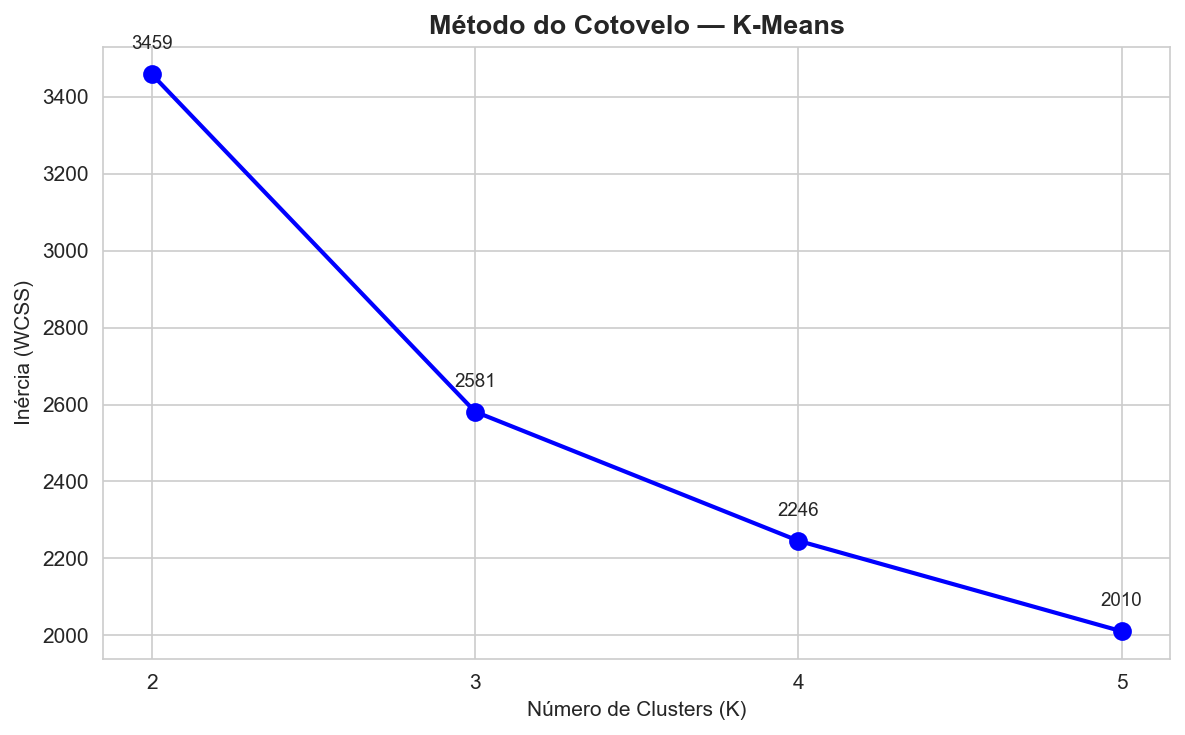
\includegraphics[width=0.7\textwidth]{graficos/06_elbow_method.png}
    \caption{Método do Cotovelo --- K-Means}
    \label{fig:elbow}
\end{figure}

\begin{figure}[H]
    \centering
    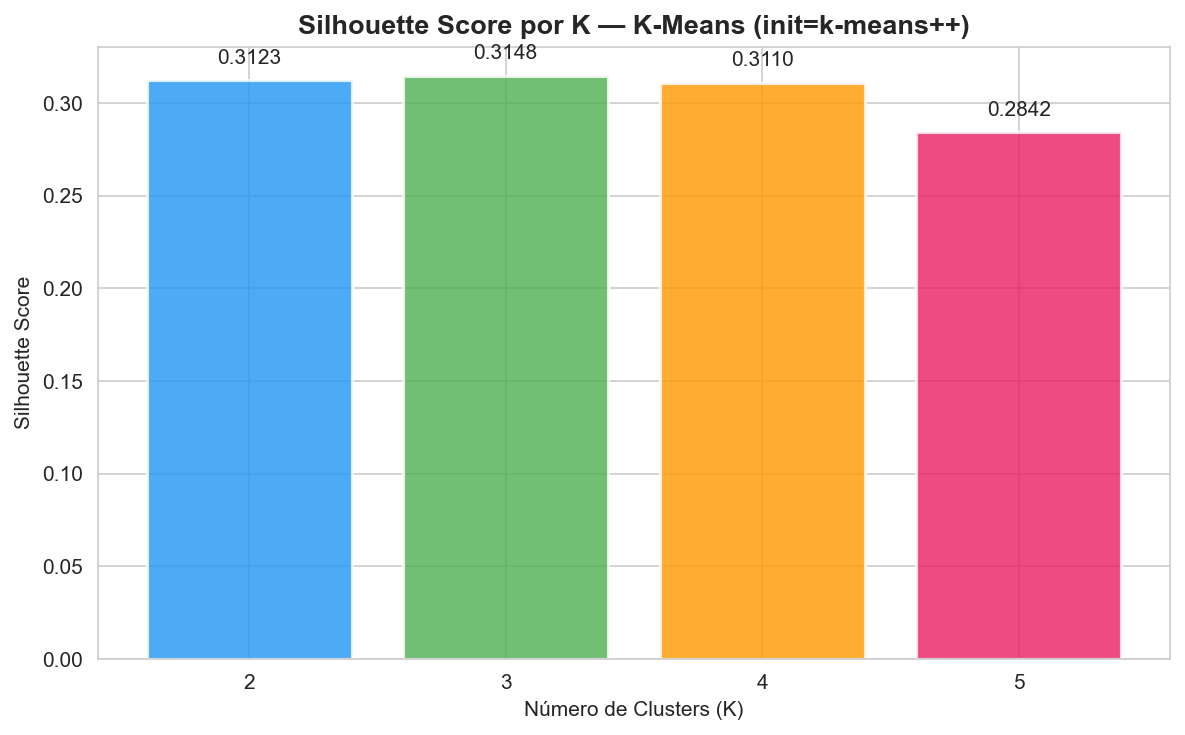
\includegraphics[width=0.7\textwidth]{graficos/07_silhouette_kmeans.png}
    \caption{Silhouette Score por K --- K-Means}
    \label{fig:silhouette_kmeans}
\end{figure}

\subsection{Agglomerative Clustering}

O modelo hierárquico foi testado com $n\_clusters \in \{2, 3, 4, 5\}$ e métodos de \texttt{linkage} (Tabela \ref{tab:agg}).

\begin{table}[H]
\centering
\caption{Resultados do Agglomerative Clustering (Top configurações)}
\label{tab:agg}
\begin{tabular}{llrrr}
\toprule
\textbf{n\_clusters} & \textbf{Linkage} & \textbf{Silhouette} & \textbf{Davies-Bouldin} & \textbf{Calinski-Harabasz} \\
\midrule
\textbf{2} & \textbf{ward} & \textbf{0.3399} & \textbf{1.1177} & \textbf{394.21} \\
2 & average & 0.3380 & 1.1396 & 402.41 \\
3 & ward & 0.2956 & 1.2849 & 447.63 \\
4 & average & 0.3071 & 1.1002 & 351.93 \\
\bottomrule
\end{tabular}
\end{table}

\textbf{Análise:} O \texttt{linkage} \textit{ward} obteve os melhores resultados. É notável que o melhor Silhouette (0.3399) ocorreu com \textbf{2 clusters}, sugerindo que a separação mais natural nos dados é binária (risco elevado vs. não-elevado). O dendrograma ilustra essa hierarquia (Figura \ref{fig:dendrograma}).

\begin{figure}[H]
    \centering
    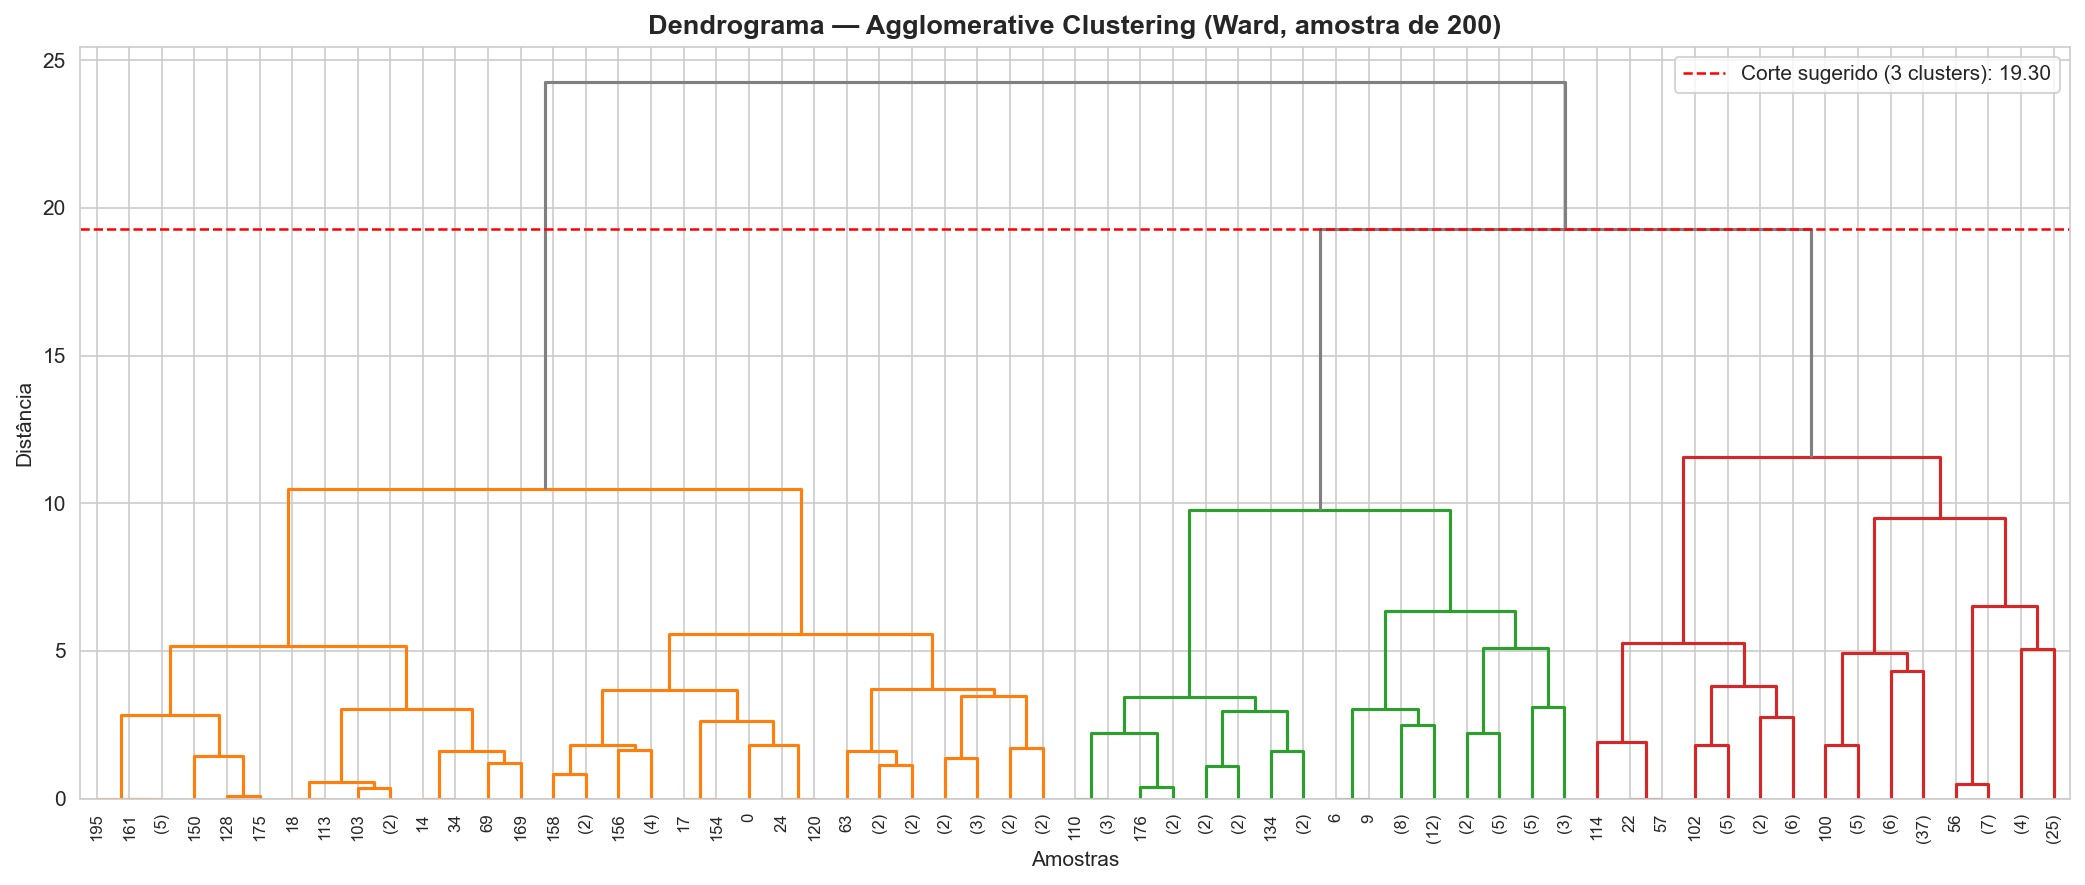
\includegraphics[width=\textwidth]{graficos/08_dendrograma.png}
    \caption{Dendrograma --- Agglomerative Clustering}
    \label{fig:dendrograma}
\end{figure}

\subsection{DBSCAN}

O DBSCAN foi testado com várias combinações de $\epsilon$ e $min\_samples$ (Tabela \ref{tab:dbscan}).

\begin{table}[H]
\centering
\caption{Resultados do DBSCAN (Amostra Selecionada)}
\label{tab:dbscan}
\begin{tabular}{lrrrrrr}
\toprule
\textbf{eps} & \textbf{min\_s} & \textbf{Clusters} & \textbf{Ruído} & \textbf{Silhouette} & \textbf{DBI} & \textbf{CHI} \\
\midrule
0.3 & 3 & 117 & 230 & 0.7864 & 0.2836 & 1308.31 \\
0.3 & 15 & 5 & 886 & 0.8901 & 0.2041 & 5305.39 \\
0.5 & 5 & 63 & 262 & 0.6159 & 0.5170 & 388.25 \\
0.7 & 10 & 20 & 332 & 0.4204 & 0.6885 & 227.70 \\
1.0 & 5 & 14 & 38 & 0.0315 & 0.8042 & 62.04 \\
\bottomrule
\end{tabular}
\end{table}

\textbf{Seleção do melhor modelo:} Configurações com Silhouette artificialmente altos classificavam até 87.5\% dos dados como ruído (886 pontos em $\epsilon=0.3$). Aplicando uma restrição de cobertura ($\le 50\%$ de ruído), o "melhor" modelo seria $\epsilon=0.3, min\_samples=3$, com 22.7\% de ruído.

\textbf{Análise crítica:} Mesmo com a restrição, o DBSCAN gerou \textbf{117 microclusters}, impedindo qualquer interpretação clínica. O \textit{K-Distance Plot} (Figura \ref{fig:kdistance}) confirma que o dataset não possui estrutura de densidade definida, tornando o DBSCAN inadequado para este cenário.

\begin{figure}[H]
    \centering
    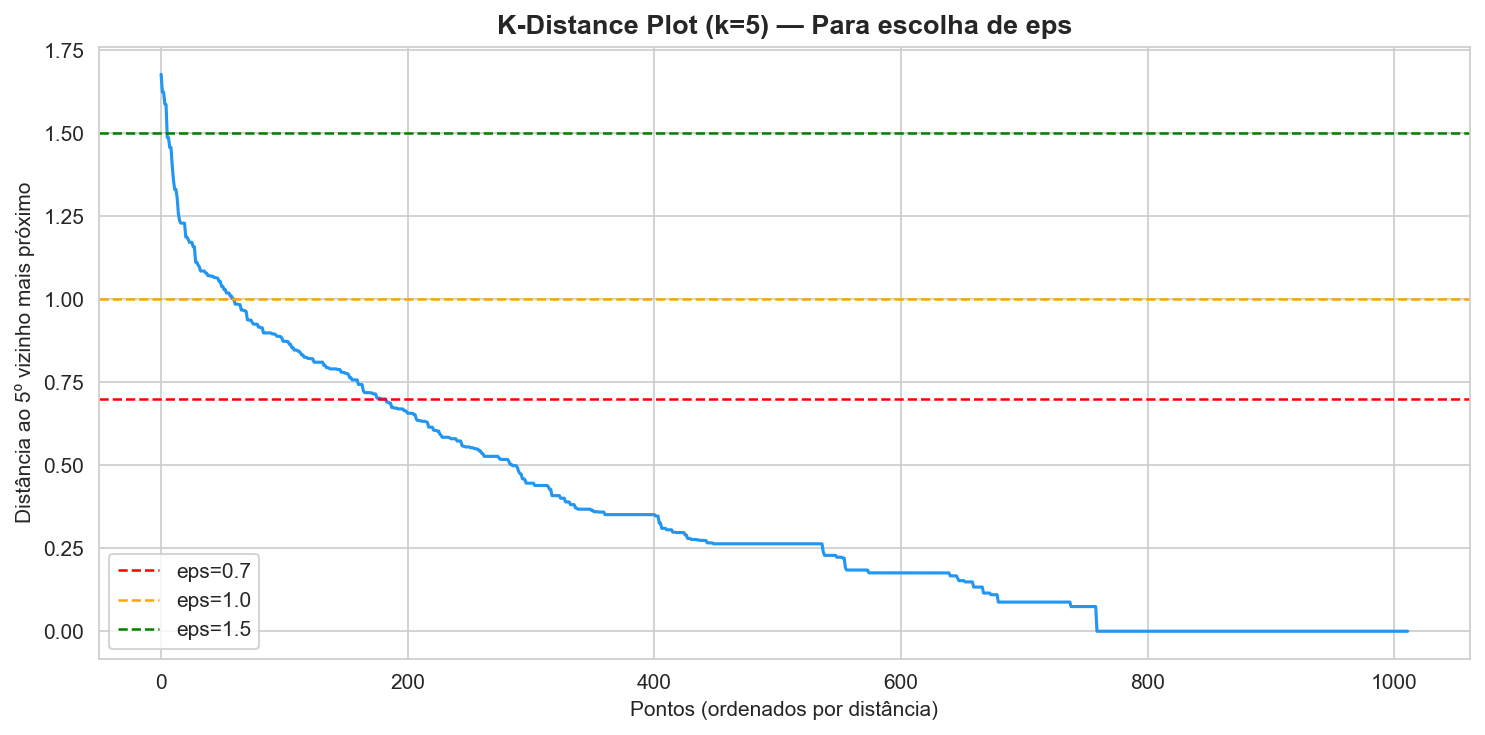
\includegraphics[width=0.7\textwidth]{graficos/09_kdistance.png}
    \caption{K-Distance Plot para escolha de eps}
    \label{fig:kdistance}
\end{figure}

\section{Avaliação Comparativa}

\subsection{Tabela Comparativa dos Melhores Modelos}

A Tabela \ref{tab:comparativa} resume a melhor configuração encontrada para cada algoritmo.

\begin{table}[H]
\centering
\caption{Comparação dos Melhores Modelos por Algoritmo}
\label{tab:comparativa}
\begin{tabular}{llrrr}
\toprule
\textbf{Algoritmo} & \textbf{Melhor Configuração} & \textbf{Silhouette} & \textbf{DBI} & \textbf{CHI} \\
\midrule
\textbf{K-Means} & K=3, init=k-means++ & 0.3148 & 1.2216 & 484.40 \\
\textbf{Agglomerative} & n\_clusters=2, linkage=ward & 0.3399 & 1.1177 & 394.21 \\
\textbf{DBSCAN} & eps=0.3, min\_samples=3 & 0.7864* & 0.2836* & 1308.31* \\
\bottomrule
\multicolumn{5}{p{0.9\textwidth}}{\footnotesize *Valores do DBSCAN elevados pela natureza do algoritmo (microclusters densos com exclusão de 22.7\% dos dados como ruído). Não diretamente comparáveis com K-Means e Agglomerative, que classificam todos os pontos.}
\end{tabular}
\end{table}

\subsection{Discussão Comparativa}

\textbf{K-Means vs. Agglomerative:} Os resultados de ambos os algoritmos são próximos em termos de Silhouette (0.31 vs. 0.34), o que é esperado dado que ambos utilizam distâncias euclidianas. O Agglomerative com 2 clusters obteve Silhouette ligeiramente superior, sugerindo que a separação binária (risco elevado vs. não-elevado) é mais nítida do que a ternária. No entanto, o K-Means com $K=3$ apresentou melhor Calinski-Harabasz (484 vs. 394), indicando que, apesar de mais difusa, a separação em 3 grupos captura mais variância inter-cluster.

\textbf{DBSCAN:} A estrutura dos dados não apresenta clusters de densidade uniforme claramente separados por regiões de baixa densidade — premissa fundamental do DBSCAN. Os dados se distribuem de forma mais difusa, favorecendo algoritmos baseados em partição.

\textbf{Conclusão da avaliação:} Para fins práticos de estratificação de risco materno, o \textbf{K-Means com K=3} é o modelo mais adequado, pois (1) classifica todas as instâncias, (2) gera 3 clusters alinhados ao número real de níveis de risco, e (3) apresenta métricas competitivas.

\begin{figure}[H]
    \centering
    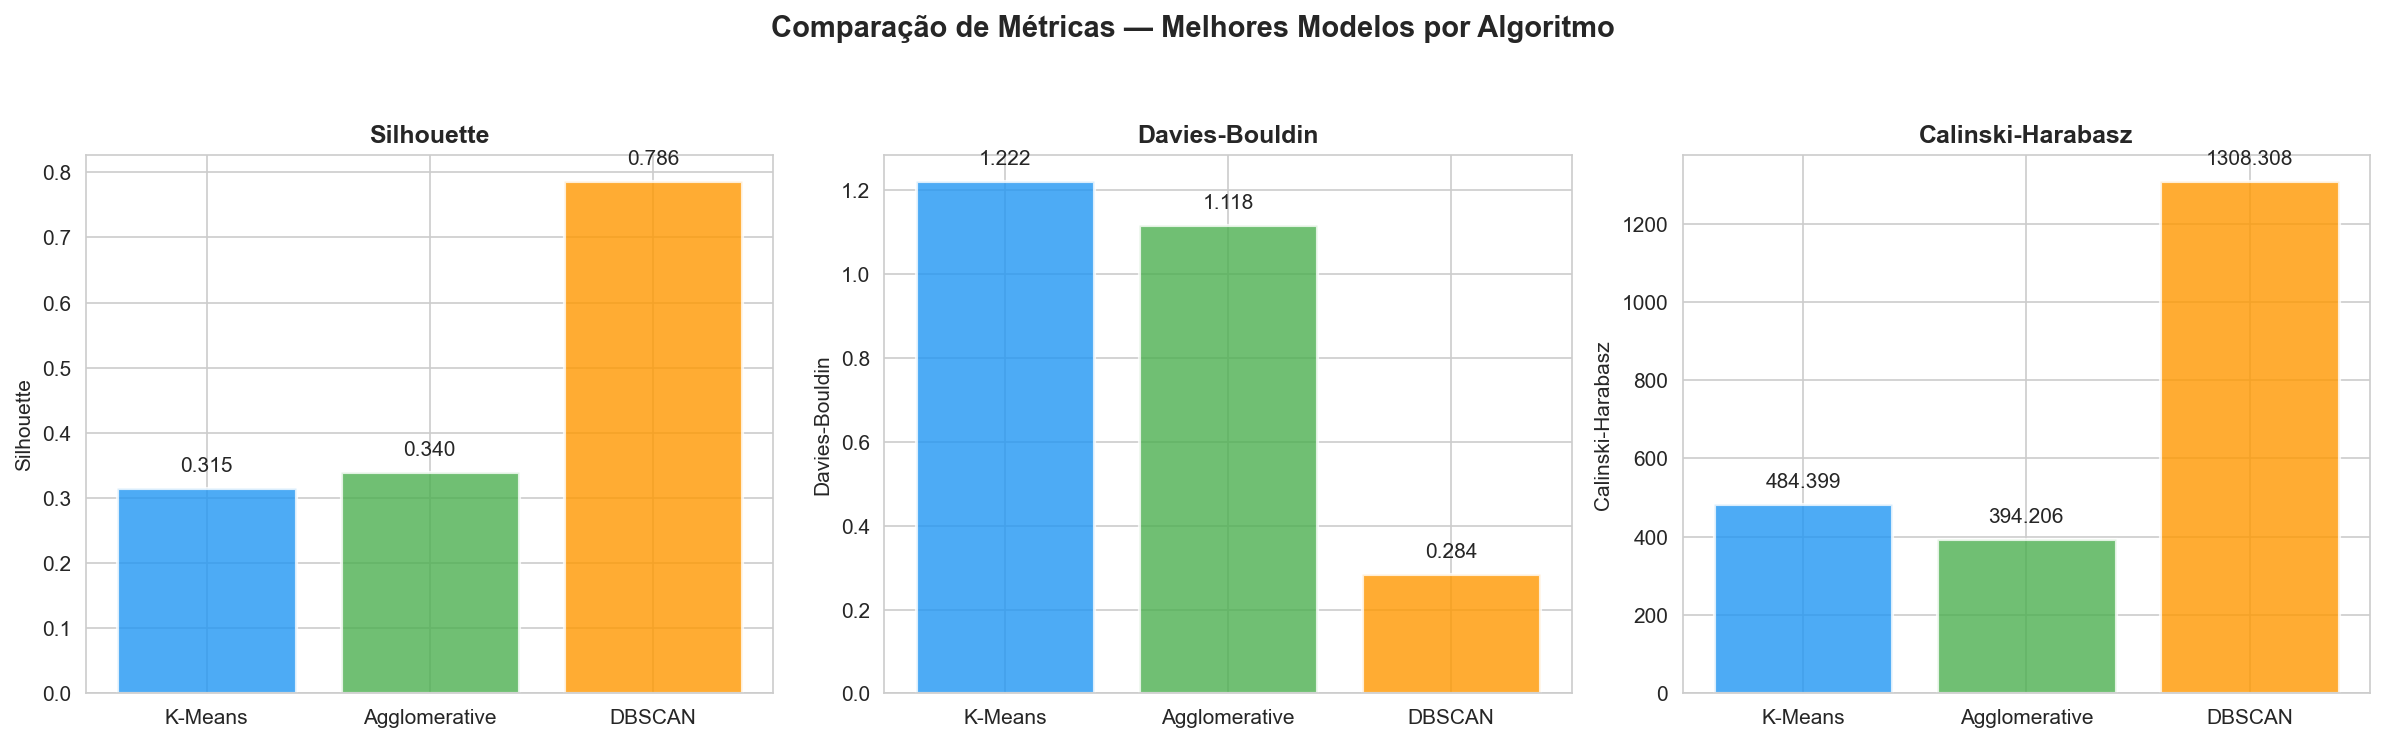
\includegraphics[width=\textwidth]{graficos/13_comparacao_metricas.png}
    \caption{Comparação de Métricas --- Melhores Modelos por Algoritmo}
    \label{fig:comparacao_metricas}
\end{figure}

\section{Interpretação dos Clusters}

\subsection{K-Means (K=3) — Melhor modelo para interpretação}

Após a clusterização, os rótulos originais (\texttt{RiskLevel}) foram reintroduzidos para avaliar a correspondência empírica (Tabela \ref{tab:contingencia_kmeans}).

\begin{table}[H]
\centering
\caption{Tabela de Contingência (Cluster $\times$ RiskLevel) --- K-Means}
\label{tab:contingencia_kmeans}
\begin{tabular}{lrrrr}
\toprule
\textbf{Cluster} & \textbf{High Risk} & \textbf{Low Risk} & \textbf{Mid Risk} & \textbf{Total} \\
\midrule
0 & \textbf{157 (77.0\%)} & 9 (4.4\%) & 38 (18.6\%) & 204 \\
1 & 59 (18.8\%) & \textbf{160 (51.1\%)} & 94 (30.0\%) & 313 \\
2 & 56 (11.3\%) & \textbf{235 (47.5\%)} & 204 (41.2\%) & 495 \\
\midrule
\textbf{Total} & 272 & 404 & 336 & 1012 \\
\bottomrule
\end{tabular}
\end{table}

\begin{table}[H]
\centering
\caption{Perfil Médio de Cada Cluster --- K-Means}
\label{tab:perfil_kmeans}
\begin{tabular}{lrrrrrr}
\toprule
\textbf{Cluster} & \textbf{Age} & \textbf{SystolicBP} & \textbf{DiastolicBP} & \textbf{BS} & \textbf{BodyTemp} & \textbf{HeartRate} \\
\midrule
0 & 45.07 & 130.39 & 89.83 & 9.50 & 98.0 & 77.13 \\
1 & 21.81 & 90.33 & 60.96 & 7.48 & 98.0 & 75.99 \\
2 & 28.76 & 120.34 & 80.76 & 7.13 & 98.0 & 72.34 \\
\bottomrule
\end{tabular}
\end{table}

\textbf{Análise dos Clusters:}
\begin{itemize}
    \item \textbf{Cluster 0 (n=204) — Alto Risco:} Capturou \textbf{77.0\% de gestantes high risk}. Perfil: idade elevada (média 45 anos), pressão arterial sistólica alta (130 mmHg) e glicose elevada (9.5 mmol/L). O algoritmo identificou o subgrupo com precisão. O perfil é consistente com pré-eclâmpsia e diabetes gestacional, \textbf{confirmando a hipótese H2}.
    \item \textbf{Cluster 1 (n=313) — Baixo Risco:} Concentra \textbf{51.1\% de gestantes low risk}. Perfil: jovens (média 22 anos), pressão baixa (90/61 mmHg) e glicose normal (7.48 mmol/L). Contudo, contém 30\% de mid risk.
    \item \textbf{Cluster 2 (n=495) — Perfil Misto:} Maior cluster, distribuição equilibrada entre low (47.5\%) e mid (41.2\%) risk. Isso revela que \textbf{low risk e mid risk são difíceis de separar}.
\end{itemize}

\begin{figure}[H]
    \centering
    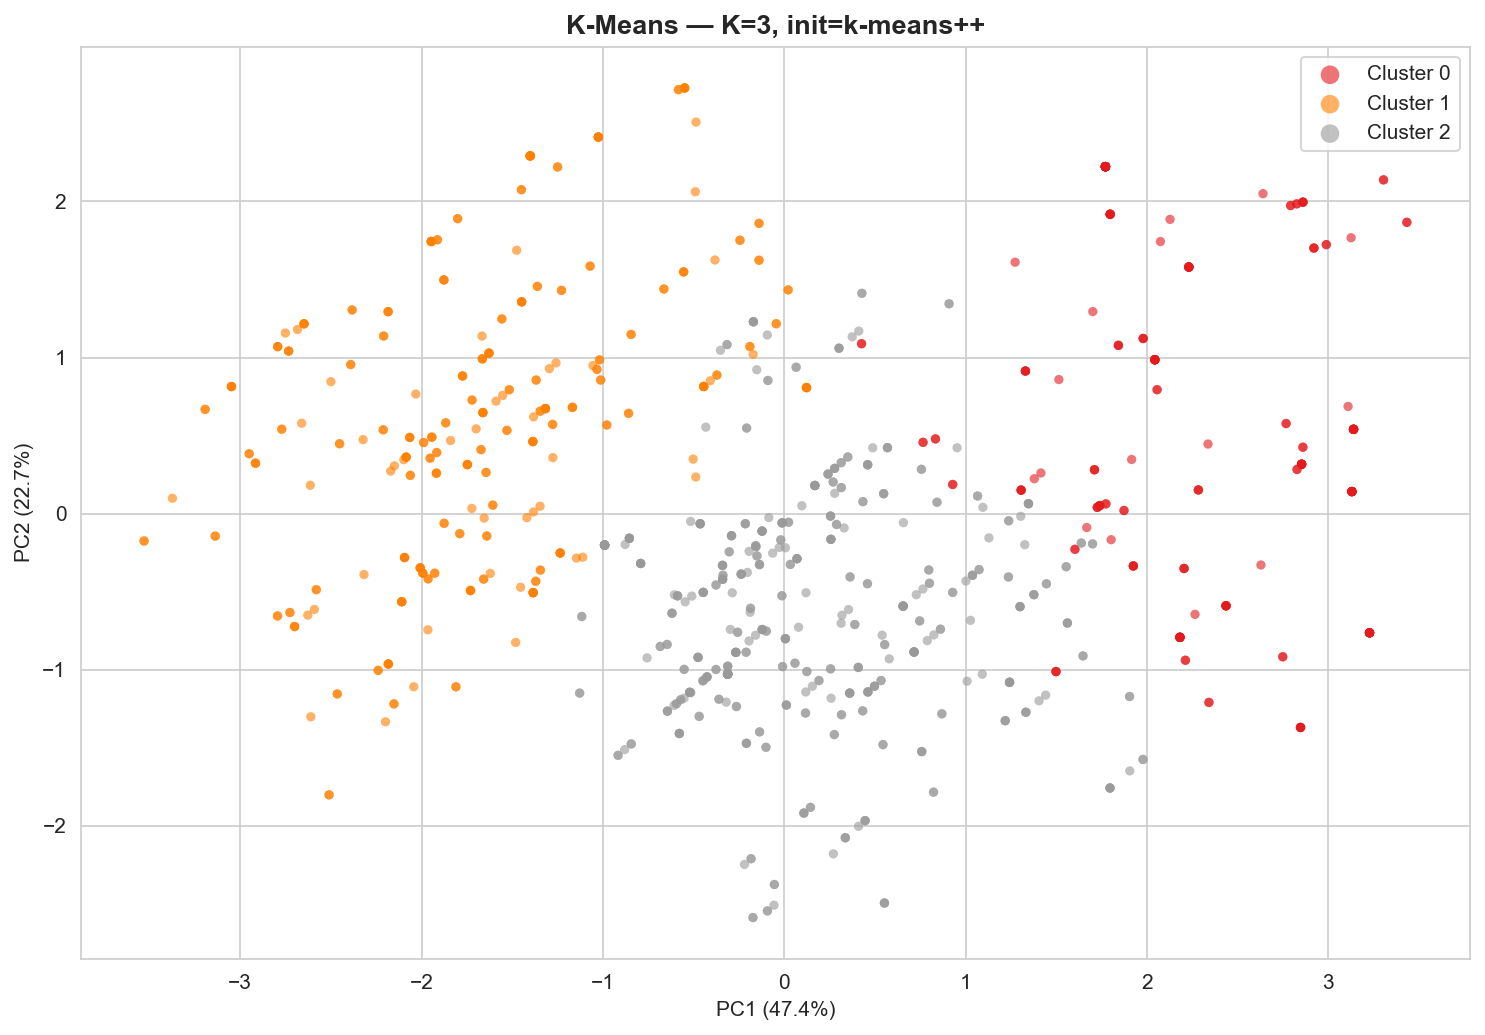
\includegraphics[width=0.8\textwidth]{graficos/10_clusters_kmeans.png}
    \caption{Clusters K-Means no espaço PCA}
    \label{fig:clusters_kmeans}
\end{figure}

\begin{figure}[H]
    \centering
    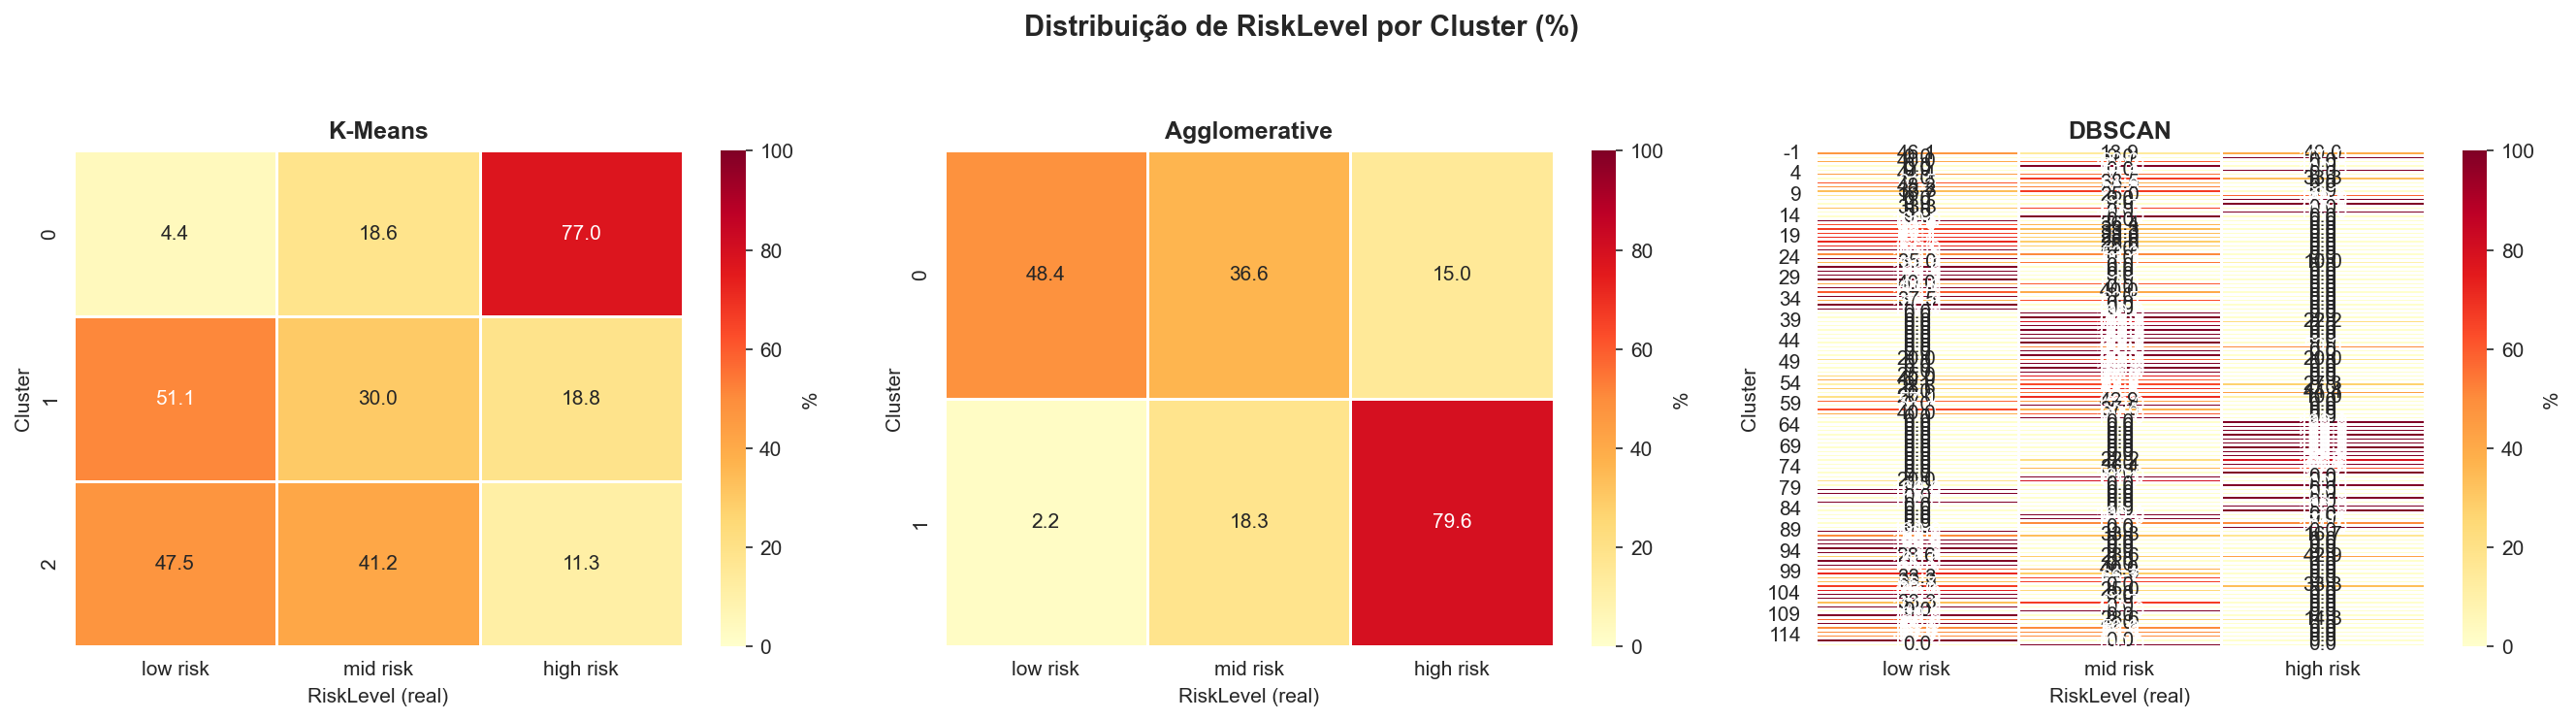
\includegraphics[width=\textwidth]{graficos/14_crosstab_heatmap.png}
    \caption{Distribuição de RiskLevel por Cluster --- Heatmap}
    \label{fig:crosstab_heatmap}
\end{figure}

\subsection{Síntese da Interpretação}

Os resultados demonstram que:
\begin{enumerate}
    \item \textbf{O K-Means com $K=3$ identifica com boa acurácia o grupo de alto risco} (77\% de pureza no Cluster 0), \textbf{confirmando H2}.
    \item \textbf{A separação entre low risk e mid risk é difícil}, sugerindo que os critérios clínicos para diferenciar esses níveis envolvem mais do que as 6 métricas disponíveis. Logo, \textbf{H1 é parcialmente refutada}.
    \item \textbf{A estrutura natural dos dados aproxima-se de uma separação binária} (alto risco vs. não-alto risco).
\end{enumerate}

\section{Conclusão}

Este trabalho investigou se algoritmos de clusterização não supervisionada conseguem agrupar gestantes em perfis de risco utilizando exclusivamente métricas fisiológicas. Os três algoritmos testados --- K-Means, Agglomerative Clustering e DBSCAN --- revelaram padrões importantes.

O \textbf{K-Means com K=3} demonstrou ser o mais adequado para a tarefa, isolando um cluster de alto risco com \textbf{77\% de pureza}, com perfil clínico coerente. Esse resultado valida parcialmente a tese de que existem padrões fisiológicos naturais que distinguem os níveis de risco, \textbf{confirmando a hipótese H2} (alto risco é o mais distinguível) e \textbf{parcialmente confirmando H1} (três agrupamentos são formados, mas com sobreposição).

A \textbf{principal limitação} observada é a dificuldade de separar gestantes de baixo e médio risco, cujas métricas fisiológicas apresentam sobreposição considerável. O \textbf{DBSCAN} mostrou-se inadequado para dados com distribuição contínua, enquanto o \textbf{Agglomerative Clustering} confirmou que a separação binária é a fronteira mais nítida.

Em resumo, os algoritmos \textbf{são eficazes para identificar o perfil de alto risco materno}, mas insuficientes para uma estratificação completa em três níveis sem informações adicionais.

\end{document}
